\documentclass[10pt,a4paper]{article}
\usepackage[a4paper,margin=1.45cm]{geometry}
\usepackage{graphicx}
\usepackage{amsmath,amssymb}
\usepackage{booktabs}
\setlength{\parindent}{0pt}
\setlength{\parskip}{1.2pt}
\pagestyle{plain}
\makeatletter
\renewcommand\section{\@startsection{section}{1}{0pt}{0.8ex plus .2ex}{0.4ex}{\normalfont\large\bfseries}}
\makeatother
\setlength{\abovedisplayskip}{3pt}\setlength{\belowdisplayskip}{3pt}
\setlength{\abovedisplayshortskip}{2pt}\setlength{\belowdisplayshortskip}{2pt}
\setlength{\textfloatsep}{5pt}\setlength{\floatsep}{4pt}\setlength{\intextsep}{4pt}\setlength{\abovecaptionskip}{2pt}\setlength{\belowcaptionskip}{0pt}
\newcommand{\ex}{\exists}
\newcommand{\fa}{\forall}
\newcommand{\Dthree}{\mathrm{D3}^{+}}
\newcommand{\Bad}{\mathit{Bad}}
\newcommand{\lt}[1]{\texttt{#1}}
\begin{document}
\fontsize{9}{10.3}\selectfont
\begin{center}
{\Large\bfseries Delegating a contract to a planner in series with an existing controller}\\[2pt]
Validated version, 27 October 2026
\end{center}

\section{Problem}

\textbf{Ports and behaviours.} A planner $M_1$ is to be written in series with an existing waypoint controller $M_2$ so that the pair meets a given contract. The ports are $\Pi=U\cup W\cup E\cup Y$. $U$ is the planner's input (here fence half-side $s$, home $h$, goal $g$); $W$ is the wire, a mission of at most $N$ items, each an item kind and a waypoint, stored as a fixed-length vector with a length field $n$; $E=E_s\cup E_d$ is the environment, with a static part $E_s$ (start position $p_0$, parameters, the controller's initial internal state) and a per-tick part $E_d$ (measured tick length $dt$, state estimates); $Y$ holds the controller's per-tick targets $y_t$. Ticks are $t\in\{0,\dots,H\}$ for a horizon $H$. A behaviour gives each port of $U$, $W$, $E_s$ one value and each port of $E_d$, $Y$ one value per tick, and we write $(u,w,e,y)$ for its values on $U,W,E,Y$. The set $\Omega$ of behaviours is the product over ports of these per-port signal spaces, and $\lnot S:=\Omega\setminus S$ for $S\subseteq\Omega$. The length field is a case split over $n\in\{1,\dots,N\}$ with the slots after $n$ left free, so a formula about the last waypoint or the polyline through the waypoints is a disjunction over $n$ (for a tube, $O(N^2)$ atoms).

\textbf{Projections.} For $X\subseteq\Pi$, two behaviours are $X$-equivalent if they agree on every port outside $X$; $\ex_X S$ is the set of behaviours $X$-equivalent to a member of $S$, and $\fa_X S:=\lnot\ex_X\lnot S$. A set $S$ is \emph{over} $Z\subseteq\Pi$ if $\ex_{\Pi\setminus Z}S=S$. We use five facts. (F0) Sets over $Z$ are closed under $\lnot,\cap,\cup$ and are over every $Z'\supseteq Z$. (F1) $\fa_X S\subseteq S\subseteq\ex_X S$, and both operators are monotone. (F2) If $S$ is over $Z$, then $\ex_X S$ and $\fa_X S$ are over $Z\setminus X$; this rests on $\ex_X\ex_{X'}=\ex_{X\cup X'}$, which holds because $\Omega$ is a product. (F3) If $C$ is over $\Pi\setminus X$, then $C\subseteq S$ iff $C\subseteq\fa_X S$, and $S\subseteq C$ iff $\ex_X S\subseteq C$ (the hypothesis is needed, as $X=\{x\}$ and $C=S=\{x=0\}$ give $\fa_X S=\emptyset$). (F4) If $C$ is over $\Pi\setminus X$, then $\ex_X(C\cap S)=C\cap\ex_X S$.

\textbf{Contracts.} A contract is a pair $(A,G)$ of subsets of $\Omega$, and a component $M\subseteq\Omega$ satisfies it, $M\models(A,G)$, iff $M\cap A\subseteq G$. PolySTL formulas have atoms $p\ge0$ and $p>0$ with $p$ a rational polynomial in the values at the current tick, the connectives $\lnot,\wedge,\vee$, and the operators $\Box_I,\Diamond_I,\mathcal U_I$ with integer windows $I\subseteq[0,H]$; a formula denotes the behaviours that satisfy it at tick $0$. Given are PolySTL formulas $A$ and $G$ over $U\cup E\cup Y$ and the controller $M_2$ over $W\cup E\cup Y$ as deterministic code with bounded loops. $A$ may mention $Y$ only through one-tick conditions such as a tracking bound, which is a closed-loop assumption discharged outside this method; an $A$ that couples ticks (a plant model) keeps the set-level results but leaves the class $\Phi$ below. The planner $M_1$ over $U\cup W$ does not exist yet. Wanted are $A_1$ over $U$, $G_1$ over $U\cup W$, $A_2$ over $W\cup E$ and $G_2$ over $W\cup E\cup Y$ with
\[(\mathrm{D1})\ A\subseteq A_1,\qquad(\mathrm{D2})\ G_1\subseteq A_2,\qquad(\Dthree)\ A\cap G_1\cap A_2\cap G_2\subseteq G.\]

\textbf{Why $\Dthree$.} The shorter condition $A\cap A_2\cap G_2\subseteq G$ does not work. $A_2\cap G_2$ is over $\Pi\setminus U$, so by F3 it is equivalent to $A_2\cap G_2\subseteq\fa_U(\lnot A\cup G)$, and since $A$ does not tie the goal $g$ to the mission, $\fa_U(\lnot A\cup G)$ contains, for the horizons considered, no target sequence that serves every goal $A$ allows; for a controller that accepts every input this forces $V=\emptyset$ (with $V$ from step 1). Only $G_1$ can relate $u$ to the mission, so the third condition must contain it. $\Dthree$ is implied by the shorter condition and by $A_2\cap G_2\subseteq G$, so it loses nothing, and it is exactly the side condition of guarantee tightening (weakening $G$ to a subset of it) that remains after the sequential composition rule that keeps both guarantees, from $A\subseteq A_1$ and $A\cap G_1\subseteq A_2$ to $(A,G_1\cap G_2)$, whose second side condition is weaker than D2. Under that weaker condition the controller's environment conditions $P$ (step 1) could stay in $A_2$ as far as they are over $W\cup E$; for $A$ and $P$ that do not mention $Y$, moving them into $G_2$, as step 2 does, gives the same planner guarantee when every $(u,e)$ allowed by $A$ admits a target outside $G$ and a larger one otherwise, and it leaves the controller's obligation unchanged (Theorem, d).

\textbf{Pointwise class.} $\Phi$ is the set of formulas $\beta\wedge\Box_{[0,H]}\alpha\wedge\bigwedge_{j=1}^{m}\Diamond_{[0,H]}\gamma_j$ in which $\beta$ is quantifier-free over the static ports $U\cup W\cup E_s$, each of $\alpha,\gamma_1,\dots,\gamma_m$ is quantifier-free over the static ports and the values of one tick, and every window equals $[0,H]$.

\section{The algorithm}

The algorithm takes $A$, $G$, $H$ and the code of $M_2$ and returns $(A_1,G_1)$, $(A_2,G_2)$ and a set $\Bad$ over $U$, or the report ``no controller guarantee''.

\begin{enumerate}\setlength{\itemsep}{1pt}\setlength{\parskip}{1pt}\setlength{\leftmargin}{1.2em}
\item \textbf{Propose the controller vocabulary} (input the code of $M_2$; output $V$ over $W$, $P$ over $W\cup E\cup Y$ and a chain $T_1\subseteq\dots\subseteq T_k$ over $W\cup E\cup Y$). From the guards and clamps of $M_2$ read $V$ (accepted item kinds, sentinel values excluded, $1\le n\le N$, leg lengths in $[\ell_{\min},\ell_{\max}]$, and, when reach depends on $dt$, a bound on the total length so that every mission in $V$ ends within $H$ ticks of the shortest tick length $P$ admits) and $P$ (ranges of $dt$ and of the parameters, including the conjuncts of $A$ that mention only $E$, for example the tick-length range of $A$ when reach depends on $dt$; leg conditions that involve the start; the initial internal state; and, when the controller's progress depends on its own estimates, one-tick tracking bounds $\lVert\hat x_t-y_t\rVert\le L_p$ between the position estimate $\hat x_t\in E_d$ and the target and $\lVert\hat v_t-\dot y_t\rVert\le L_v$ for the velocity estimate $\hat v_t$ and the target velocity $\dot y_t$, added to $A$ as well). $T_j$ says that at every tick the target is finite and lies within $\rho_j$ of the polyline from the start through the waypoints, and that some tick brings it within $\eta$ of the last waypoint. $\rho_1$ is the largest distance to the polyline observed when $M_2$ runs on a fixed finite list of test legs with nominal inputs, rounded down to the grid of the chain (no valid tube is thinner than that), and $\rho_j:=\rho_1+(j-1)\kappa$ for a fixed step $\kappa$ and length $k$. This is a proposal step whose output is trusted for nothing, because step 2 checks it.
\item \textbf{Certify} (input $M_2$, $V$, $P$, the chain and $H$; output $j^*$, $A_2$, $G_2$ or the report). Decide $M_2\cap V\cap P\subseteq T_j$ by bounded model checking of the code unrolled over the horizon $[0,H]$ of $A$ and $G$, since a guarantee certified over fewer ticks says nothing about the later ones. As $T_j\subseteq T_{j+1}$, the certified indices form an up-set of $\{1,\dots,k\}$, and binary search finds the least certified index $j^*$ with $\lceil\log_2k\rceil+1$ checks, provided every check returns a definite answer; a check that times out counts as not certified, which keeps soundness, but $j^*$ is then only the least index whose check returned. Under IEEE semantics each check is a finite satisfiability question; read over the reals it needs semialgebraic code (Section 5). If no index is certified, stop with the report. Otherwise set $A_2:=V$ and $G_2:=\lnot P\cup T_{j^*}$. Provided $M_2$ does not read $U$, a guarantee $G_2'$ mentioning $U$ gains nothing, because $M_2\cap A_2$ is over $\Pi\setminus U$, so by F3 $M_2$ also meets $\fa_U G_2'\subseteq G_2'$, which gives a $G_1$ at least as large.
\item \textbf{Planner assumption} (input $A$; output $A_1$ over $U$). $A_1:=\ex_{E\cup Y}A$.
\item \textbf{Planner guarantee} (input $A,G,A_2,G_2,H$; output $G_1$ over $U\cup W$).
\[G_1:=A_2\cap\fa_{E\cup Y}(\lnot A\cup\lnot A_2\cup\lnot G_2\cup G).\]
Timed operators are converted first. A deadline of $D$ seconds becomes a tick window that makes $G$ stronger and $A$ weaker, so Diamond windows in $G$ and Box windows in $A$ become $[0,\lfloor D/dt_{\max}\rfloor]$, and Box windows in $G$ and Diamond windows in $A$ become $[0,\lfloor D/dt_{\min}\rfloor]$, where $[dt_{\min},dt_{\max}]$ is the tick-length range of $A$; the loss grows with $dt_{\max}/dt_{\min}$. Unrolling over $[0,H]$ then turns $A,G,V,P,T_{j^*}$ into quantifier-free real arithmetic over samples, the projection becomes one block of universal quantifiers over the $(H+1)(|E_d|+|Y|)+|E_s|$ sampled environment and target variables with the $|U|+|W|$ static variables free, and real quantifier elimination returns an equivalent quantifier-free polynomial formula over $U\cup W$, a PolySTL formula without temporal operators read at tick $0$. Its cost is singly exponential in the number of eliminated variables for a fixed number of free variables \cite{bpr} and doubly exponential with cylindrical algebraic decomposition \cite{collins}. $U$ is static because with per-tick $U$ the elimination of the static environment ports, shared by all ticks, can produce atoms relating values of $U$ at different ticks, which PolySTL cannot express.

When $A,P,T_{j^*},G\in\Phi$ the elimination does not depend on $H$. Since $\lnot G_2=P\cap\lnot T_{j^*}$, at a mission in $V$ the condition splits into $A\cap\lnot P\subseteq G_i$ and $A\cap T_{j^*}\subseteq G_i$ for each conjunct $G_i$ of $G$, and $\lnot P$ splits into one branch per negated conjunct of $P$. Each piece is an implication $\varphi\to\Box c$ or $\varphi\to\Diamond d$ with $\varphi\in\Phi$, decided over one tick's values by the following lemma. \emph{Pointwise lemma.} Fix the static values, let $Z$ be the set of one tick's values of $E_d\cup Y$, let $\alpha,\gamma_1,\dots,\gamma_m,c,d\subseteq Z$ and read $\varphi=\Box\alpha\wedge\bigwedge_{j\le m}\Diamond\gamma_j$ over signals $z:\{0,\dots,H\}\to Z$. If $H\ge m$, then $\varphi\to\Box c$ holds for every signal iff $\alpha=\emptyset$, or $\alpha\cap\gamma_j=\emptyset$ for some $j$, or $\alpha\subseteq c$. If $H+1\ge m$, then $\varphi\to\Diamond d$ holds for every signal iff $\alpha\subseteq d$ or $\alpha\cap\gamma_j\subseteq d$ for some $j$. Here $m$ counts the Diamonds of the antecedent after the split, that is $m_A+m_T$ for $A\wedge T$ and $m_A+1$ for a branch of $\lnot P$ that contributes a Diamond, with $m_A$ and $m_T$ the numbers of Diamonds in $A$ and $T_{j^*}$. A static conjunct $\beta$ of $\varphi$ adds the disjunct $\lnot\beta$, and for a static conjunct $\beta_G$ of $G$ the implication $\beta\wedge\varphi\to\beta_G$ holds iff $\lnot\beta$, or $\varphi$ is unsatisfiable ($\alpha=\emptyset$ or some $\alpha\cap\gamma_j=\emptyset$), or $\beta_G$. The proof puts a witness of $\gamma_j$ on tick $j-1$ and a violating value on the other ticks (for the Box part tick $m$ must exist; the bound is tight). All windows must equal $[0,H]$, since with mismatched windows the formula is unsound; for one Diamond on each side, with window $[0,\theta_1]$ in the antecedent and $[0,\theta_2]$ in the consequent, it stays valid if $\theta_1\le\theta_2$ and becomes ``$\alpha\subseteq d$ or $\alpha\cap\gamma=\emptyset$'' if $\theta_1>\theta_2$, so a goal deadline is discharged only by a tube that reaches by that deadline. A converted deadline window shorter than $H$ therefore leaves $\Phi$. As a consequence, instance checks unrolled over $m+1$ ticks are complete for $\Phi$.

For a convex polygonal fence $\{z:n_i\cdot z\le b_i\}$ and a tube in a norm $\lVert\cdot\rVert$ with dual norm $\lVert\cdot\rVert_*$ no solver is needed, because the largest value of $n\cdot z$ over the $\rho$-neighbourhood of a segment $[a,b]$ is $\max(n\cdot a,n\cdot b)+\rho\lVert n\rVert_*$, so the fence part of $G_1$ asks every waypoint to lie in the fence with facet $i$ moved inward by $\rho\lVert n_i\rVert_*$, and the set of admissible starts adds its own support value. The elimination splits per leg, since each fence and tube condition involves the two endpoints of one leg only, so a mechanised call sees the coordinates of one leg and $U$ instead of all $5+2N$ free variables.
\item \textbf{Realizability} (input $A_1,G_1$; output $\Bad$ over $U$). $\Bad:=A_1\cap\lnot\ex_W G_1$, decided by elimination of the same kind; report a vacuous query if $A_1=\emptyset$. If $\Bad=\emptyset$, every input allowed by $A$ has a mission meeting $G_1$; otherwise $\Bad$ is exactly the set of inputs that no mission serves under this controller guarantee. Within the chain, no certified member gives a smaller $\Bad$. A smaller $\Bad$ needs a guarantee of a different shape (for example one-sided at corners), a smaller $V$ or a larger $P$, or the code inlined.
\end{enumerate}
Given step 1 and complete decision procedures with fixed variable orders, steps 2--5 are deterministic.

\textbf{What is known and what is new.} Steps 3--4 are the assume--guarantee quotient by the controller contract, projected onto the planner's ports. A planner over $U\cup W$ implements $(A_1,G_1)$ iff it implements the quotient $(A,G)/(A_2,G_2)$ of Incer et al.\ \cite{quot}, whose closed form is also recovered for hypercontracts \cite{hyper}; equivalently, $G_1\cup\lnot A_1$ is the weakest assumption \cite{gpb} of the most permissive implementation $\lnot A_2\cup G_2$ of the controller contract, while that of the code itself is $G_1^x:=\fa_{E\cup Y}(\lnot A\cup\lnot M_2\cup G)$, and inlining the code ($P:=\Omega$, $T:=M_2$) gives $G_1=V\cap G_1^x$. For this port typing, steps 3--4 are the input--output quotient of Pacti \cite{pacti}, whose missing component gets inputs $U$ and outputs $W$. Damera, Matheu and Baras \cite{dmb} treat delegation as a quotient of STL contracts over a common signal space without restricting the alphabet. Maximality (e), realizability (f) and hiding (c) are the adjunction of the quotient, the $\forall u\,\exists w$ reading of the projection and the hiding rule, and binary search over a fixed chain of candidates checked by a verifier is the idea of Houdini \cite{houdini}. What is new is modest. First, the pointwise lemma, which makes the universal projection over the free per-tick signals independent of the horizon for $\Phi$; it is elementary, and we did not find it stated in the contract literature we consulted. Second, Pacti's input--output quotient carried out exactly, by real quantifier elimination, for a temporal (PolySTL) contract, with the output a static semialgebraic set over $(u,w)$ (Pacti eliminates by polyhedral refinement over static formulas; Section 4 eliminates by hand). Third, the certified step from code to a guarantee whose size does not depend on the code, with the bookkeeping that keeps the obligation of $M_2$ fixed while $P$ moves into the guarantee. Fourth, a precise account of what is lost by not inlining the code (Section 3).

\section{Correctness}

\textbf{Theorem.} (a) $A_1$ is over $U$, $G_1$ over $U\cup W$, $A_2$ over $W$ and $G_2$ over $W\cup E\cup Y$. (b) D1, D2 and $\Dthree$ hold. (c) If $M_1\models(A_1,G_1)$ and $M_2\models(A_2,G_2)$, then $M_1\cap M_2\models(A,G)$ and $\ex_W(M_1\cap M_2)\models(A,G)$. If moreover $M_1$ answers every input ($\ex_W M_1=\Omega$), $M_2$ accepts every $(w,e)$ with $w\in V$ ($V\subseteq\ex_Y M_2$) and $A$ is over $U\cup E$, then $A\subseteq\ex_{W\cup Y}(M_1\cap M_2)$, so the composite has a behaviour for every $(u,e)$ allowed by $A$ and (c) is not vacuous; when $A$ holds a tracking bound over $Y$, the composite's own targets can falsify $A$, and non-vacuity then rests on that closed-loop assumption. (d) $M_2\models(A_2,G_2)$ iff $M_2\cap V\cap P\subseteq T_{j^*}$, which step 2 decides under the semantics fixed here. Every port ranges over the IEEE doubles embedded in $\mathbb R$, atoms are evaluated exactly on those values, $T_j$ requires finite outputs, the initial internal state of $M_2$ is a port of $E_s$ constrained by $P$ or fixed by $A$ (ArduPilot starts the first leg at a stopping point computed from the estimates), and the model-checking encoding (compiler model, undefined behaviour, library calls) is the trusted base. Steps 3--5 computed over all reals are then conservative, since the universal projection over $\mathbb R^n$ is contained in the one over doubles and $A_1$ over $\mathbb R^n$ contains $A_1$ over doubles, so D1 and (c) still hold, while (e) and (f) hold for the real relaxation. (e) Every $G_1'$ over $U\cup W$ with $G_1'\subseteq A_2$ and $A\cap G_1'\cap A_2\cap G_2\subseteq G$ satisfies $G_1'\subseteq G_1$. $G_1$ is unsaturated, and its saturation $G_1\cup\lnot A_1$ is the largest guarantee under the weaker side condition $A\cap G_1'\subseteq A_2$, with the same implementations, so the planner's obligation is the same. Among the certified members of the chain, $T_{j^*}$ gives the largest $G_1$ and the smallest $\Bad$ (with timeouts, among the members whose check returned). (f) If $W$ is nonempty, a planner $M_1$ with $\ex_W M_1=\Omega$ and $M_1\models(A_1,G_1)$ exists iff $\Bad=\emptyset$.

As $G_1\supseteq V\cap\lnot A_1$, the test $G_1\neq\emptyset$ says nothing; instead, $A_1\cap G_1\neq\emptyset$ iff some $u\in A_1$ and $w\in V$ have $A\subseteq P$ and $A\cap T_{j^*}\subseteq G$ at $(u,w)$, when $A$ and $P$ do not mention $Y$ and every $(u,e)$ allowed by $A$ admits a target outside $G$. The test that matters is $\Bad=\emptyset$.

\textbf{Proof.} Write $K:=\lnot A\cup\lnot A_2\cup\lnot G_2\cup G$ and $M:=M_1\cap M_2$. (a) F2 applied to $A$ and to $K$, and F0. (b) D1 is F1, D2 holds by construction, and $G_1\subseteq\fa_{E\cup Y}K\subseteq K=\lnot(A\cap A_2\cap G_2)\cup G$ by F1 gives $\Dthree$. (c) $M\cap A\subseteq M_1\cap A_1\subseteq G_1\subseteq A_2$ by D1 and D2, hence $M\cap A\subseteq M_2\cap A_2\subseteq G_2$, hence $M\cap A\subseteq A\cap G_1\cap A_2\cap G_2\subseteq G$ by $\Dthree$; as $A$ and $G$ are over $\Pi\setminus W$, F4 gives $\ex_W M\cap A=\ex_W(M\cap A)$ and F3 gives $\ex_W(M\cap A)\subseteq G$. For non-vacuity, $A=A\cap\ex_W M_1=\ex_W(A\cap M_1)\subseteq\ex_W(M_1\cap V)\subseteq\ex_W(M_1\cap\ex_Y M_2)=\ex_W\ex_Y M$ by F4 (with $A$ over $\Pi\setminus W$ and $M_1$ over $\Pi\setminus Y$), $M_1\cap A\subseteq G_1\subseteq V$ and F2. (d) $M_2\cap V\subseteq\lnot P\cup T_{j^*}$ iff $M_2\cap V\cap P\subseteq T_{j^*}$. (e) $A\cap G_1'\cap A_2\cap G_2\subseteq G$ iff $G_1'\subseteq K$ iff $G_1'\subseteq\fa_{E\cup Y}K$ by F3, as $G_1'$ is over $\Pi\setminus(E\cup Y)$; with $G_1'\subseteq A_2$ this is $G_1'\subseteq G_1$. If $T\subseteq T'$ then $\lnot P\cup T\subseteq\lnot P\cup T'$, so the $K$ and $G_1$ built from $T'$ are contained in those built from $T$ (F1), and $\Bad$ grows. (f) If $\Bad=\emptyset$, take $M_1:=G_1\cup\lnot A_1$; then $\ex_W M_1\supseteq\ex_W G_1\cup\lnot A_1\supseteq A_1\cup\lnot A_1=\Omega$ by F1 and F0, and $M_1\cap A_1\subseteq G_1$. Conversely, $A_1=A_1\cap\ex_W M_1=\ex_W(A_1\cap M_1)\subseteq\ex_W G_1$ by F4 and F1. \hfill$\square$

The set-level content of the Theorem (all of (a)--(f) except the number semantics of (d)), the quotient identity, the pointwise lemma with its tightness and window counterexamples, the deadline rule for integer tick lengths and F2--F4 over a product of ports are machine-checked in \lt{notes/validation/Deleg.lean} (with $A$ over $U\cup E$, the case with $Y$ a separate lemma, and the lemma without the static conjunct), 56 theorems with no \lt{sorry}, compiled in the directory \lt{lean} by \lt{lake env lean /Users/ryan/Research/delegate/notes/validation/Deleg.lean}.

\textbf{Conservatism.} Let $G_1^x$ be the exact planner guarantee of Section 2. If $M_2$ is certified, then on inputs in $A_1$ the missions accepted by $G_1$ are among those accepted by $G_1^x\cap V$, and the loss $\Delta$, the set of pairs $(u,w)$ with $u\in A_1$ accepted by $G_1^x$ but not by $G_1$, splits into three disjoint parts, $\Delta=\Delta_V\cup\Delta_P\cup\Delta_T$, where $\Delta_V$ holds the missions outside $V$ that the code handles correctly, $\Delta_P$ the missions in $V$ at inputs where $A$ allows an environment outside $P$ at which some target breaks $G$, and $\Delta_T$ the missions where every allowed environment satisfies $P$ and some target sequence inside $T_{j^*}$ breaks $G$ but none that $M_2$ produces does. Only $\Delta_T$ depends on the radius $\rho:=\rho_{j^*}$. For a convex fence with facets $n_i\cdot z\le b_i$ and $\lVert n_i\rVert_*=1$, let $\mathrm{sp}_S(n):=\sup\{n\cdot z:z\in S\}$, let $\mathcal Y(w,e)$ be the set of targets the code visits, and let $\rho_{\min}$, the true deviation, be the supremum over valid inputs of the distance from $\mathcal Y$ to the polyline. The tube $T_\rho$ of radius $\rho$ around the polyline has $\mathrm{sp}_{T_\rho}(n)=\max_v n\cdot v+\rho$ over the polyline vertices $v$, so the margin lost at facet $i$ is
\[\Delta_i:=\mathrm{sp}_{T_\rho}(n_i)-\mathrm{sp}_{\mathcal Y}(n_i)\in[\rho-\rho_{\min},\ \rho+\mathrm{dist}(v^*,\mathcal Y)],\]
with $v^*$ the maximising vertex. As $\rho\to\rho_{\min}$ the lower end goes to $0$ but the upper end goes to $\rho_{\min}+\mathrm{dist}(v^*,\mathcal Y)>0$; the loss vanishes only if the controller deviates outward by the full $\rho_{\min}$ at every maximising vertex, which a controller that cuts corners inward does not. The repair is a shape-aware chain. ArduPilot's blended corner target $w_i-r_1\nu_1+r_2\nu_2$ (unit leg directions $\nu_1,\nu_2$, distance $r_1$ left on the first leg, distance $r_2$ covered on the second, leg lengths $\ell_1,\ell_2$) lies in the triangle $\mathrm{conv}(w_{i-1},w_i,w_{i+1})$ whenever $r_1/\ell_1+r_2/\ell_2\le1$, so the guarantee ``target within $\rho_j'$ of the union of these triangles'' has support value $\max_v n\cdot v+\rho_j'$, the fence condition keeps its form, and $\rho_j'$ covers only the along-track overshoot, provided step 2 also certifies $r_1/\ell_1+r_2/\ell_2\le1$. In the worked example of Section 4 (E4) at $s=50$ with $\rho'=\eta=0.5$ and the goal on a coordinate axis, the goal part of $\Bad$ moves from $\lVert g\rVert_\infty>50.5$ to $\lVert g\rVert_\infty>52$ ($53$ for a controller that reaches $w_2$ exactly and stays in the fence) and the home part from $\lVert h\rVert_\infty>47$ to $\lVert h\rVert_\infty>48.5$ ($49$ for the start disc alone). Hence step 5 says that within the chain no certified member gives a smaller $\Bad$ and a smaller one needs a different shape, a smaller $V$, a larger $P$ or the code inlined.

\section{Validation}

\begin{figure}[b]
\centering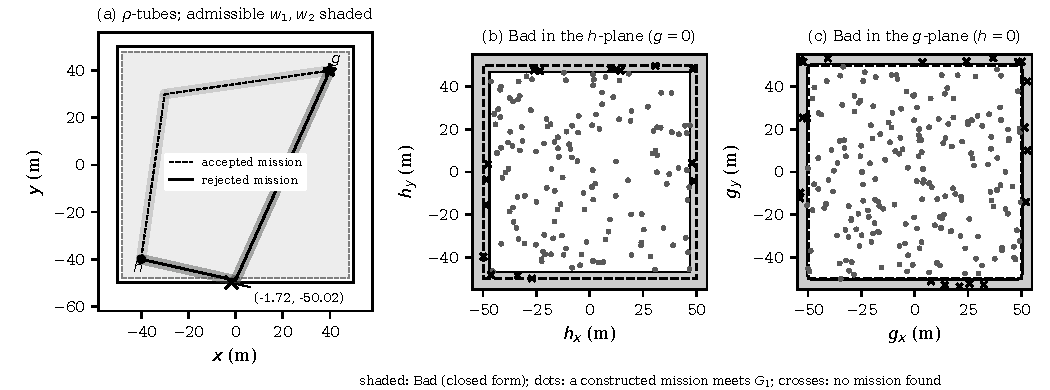
\includegraphics[width=0.86\textwidth]{figs/validation/e4_geometry_bad.pdf}
\caption{Worked example at $s=50$, showing the tubes of an accepted and a rejected mission (a) and the closed-form $\Bad$ (shaded) against constructed missions (dots) and failed searches (crosses) in the home plane (b) and the goal plane (c).}\label{geo}
\end{figure}
\begin{table}[b]
\centering\scriptsize
\begin{tabular}{lrrrrrrr}
\toprule
horizon $H$ (ticks) & 2 & 4 & 8 & 16 & 32 & 64 & 128\\
\midrule
reach part of $T_{j^*}$ & fails & fails & holds & holds & holds & holds & holds\\
step 2 total, 8 workers (s) & 8.7 & 13.3 & 17.7 & 25.9 & 39.4 & 70.6 & 150.0\\
step 2 total, sequential (s) & 6.60 & 8.58 & 12.66 & 18.54 & 31.70 & & \\
planner check R4, $u\in A_1$ free (s) & 0.339 & 0.384 & 0.356 & 0.336 & 0.355 & & \\
monolithic R4, $u$ free, fair order (s) & 0.04 rej. & 9.03 & 12.04 & 18.52 & 32.20 & & \\
monolithic R4, $u$ free, original order (s) & 0.0 rej. & & 600.1 t/o & & & & \\
monolithic R4, one fixed $u$, mean of 8 (s) & 0.009 & 0.016 & 0.025 & 0.046 & 0.093 & & \\
\bottomrule
\end{tabular}
\caption{The tube checks $j=8,4,2,1$ give $j^*=2$ and $\rho_{j^*}=1.00$\,m at every horizon, step 2 certifies only from $H=8$ where reach holds (at $H=2,4$ its time ends in the report), and every monolithic check accepts R4 from $H=4$ except the original order, which times out (t/o); at $H=2$ the fixed-input mean mixes 3 accepts and 5 rejects.}\label{tab}
\end{table}
\begin{figure}[t]
\centering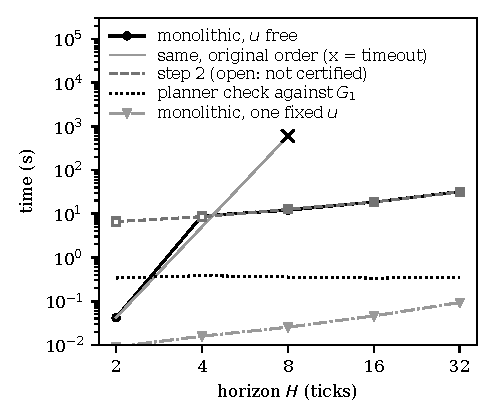
\includegraphics[width=0.48\textwidth]{figs/validation/e3_time_vs_H.pdf}\hfill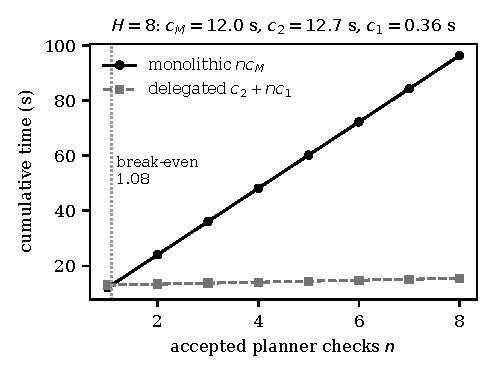
\includegraphics[width=0.48\textwidth]{figs/validation/e3_cumulative_R.pdf}
\caption{Check times against the horizon, sequential (left), and cumulative cost at $H=8$ against the number of accepted planner checks sharing one controller certification (right).}\label{cost}
\end{figure}
\begin{figure}[t]
\centering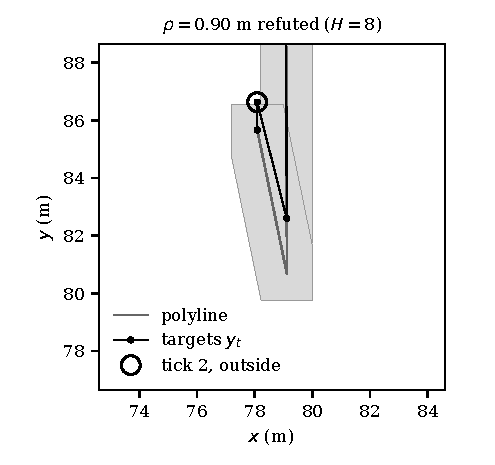
\includegraphics[width=0.48\textwidth]{figs/validation/e2_counterexample.pdf}\hfill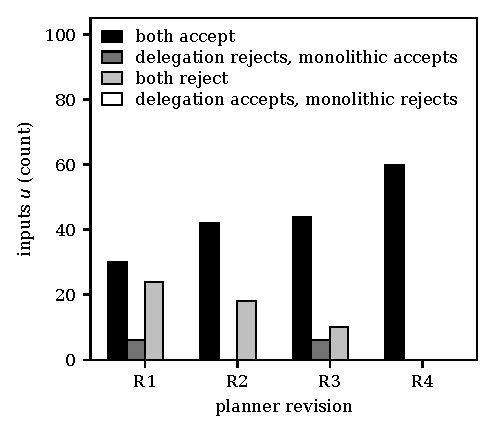
\includegraphics[width=0.48\textwidth]{figs/validation/e1_end_to_end.pdf}
\caption{The step-2 counterexample for $\rho=0.90$\,m, whose target leaves the tube at tick 2 (left), and the end-to-end verdicts of delegation and the monolithic check for 60 inputs per revision (right).}\label{small}
\end{figure}

\textbf{Controller model.} $M_2$ is one 34-line function (\lt{scripts/vcore.py}) that runs unchanged on floats and on terms of the SMT solver Z3 5.3.1. From the ArduPilot waypoint navigator it keeps the target advance along $p_0\to w_1\to w_2$, a speed cap of 40\,m/s and an acceleration cap of 18\,m/s$^2$ with trapezoidal braking onto $w_2$, the fast-waypoint handover inside the 2\,m waypoint radius with the rest of the first leg blended out over two ticks (the only deviation from the polyline), guards that hold the target at $p_0$ for legs outside $[\ell_{\min},\ell_{\max}]=[5,100]$\,m or points outside the upload box of half-side 100\,m, and the clamp of $dt$ into $[0.5,1.5]$\,s. It deviates in four recorded ways. Kinematics use the nominal tick of 1\,s and a clamped tick is held (with $dt$ in the advance, every encoding stayed unknown at 120\,s per tick); leg fractions advance by speed times tick over the upper end of a 10\,m length class, so the target is linear in $(w,p_0)$ on each branch; geometry uses the infinity norm (the Euclidean blend query was out of reach); and there are no state estimates, so reach does not depend on tracking (Section 5).

\textbf{Instance.} Here $u=(s,h,g)$, $A:=25\le s\le50\wedge\lVert h\rVert_\infty\le s-3\wedge\lVert g\rVert_\infty\le s+0.5\wedge\lVert p_0-h\rVert_\infty\le1\wedge\Box(0.9\le dt\le1.1)$ and $G:=\Box(y\in[-s,s]^2)\wedge\Diamond(\lVert y-g\rVert\le3)$; goals up to 0.5\,m outside the fence let a faulty planner really leave it. Step 1 reads $V$ and $P$ from the guards and the clamp ($P$ keeps $[0.5,1.5]$\,s, which contains the range of $A$; $V$ has no total-length bound, so step 2 finds the horizon at which every mission finishes), takes $\eta=0.5$\,m, observes 0.95\,m on 42 test legs and sets $\rho_j=0.95+0.05(j-1)$, $k=8$. Steps 3--5 in closed form give $G_1:=V\wedge(\lnot A_1\vee[\mathrm{(ii)}\wedge\mathrm{(iii)}\wedge\mathrm{(iv)}])$ with (ii) $6\le\lVert w_1-h\rVert_\infty\le99$, (iii) $\lVert w_1\rVert_\infty,\lVert w_2\rVert_\infty\le s-\rho_{j^*}$, (iv) $\lVert w_2-g\rVert\le2.5$, and $\Bad=\emptyset$ iff $\rho_{j^*}\le1.268$. Planner R1 flies from $h$ to $g$ via the midpoint, R2 clips $g$ into the fence shrunk by $\rho_{j^*}$, R4 adds a branch that puts $w_1$ 20\,m from $h$ towards the centre when $\lVert h-w_2\rVert_\infty<12$, and R3 is R4 with the margin of the wrong sign. The monolithic check composes the code of $M_1$ and $M_2$ over $[0,H]$ with $u$ symbolic (or fixed) and the query $A\wedge\lnot G$, by the same bounded model checking as step 2, exhaustive path enumeration in which Z3 prunes infeasible branches and decides every property atom on every feasible path and a timeout is never a verdict; the property queries differ in kind (E3).

\textbf{Results.} All soundness checks pass, including that R1, R2 and R3 fail the planner check. \emph{E1.} Against Z3 at $H=1$ with the controller replaced by $G_2$ (complete by the pointwise lemma, $H\ge m=1$), all 60 random input--mission pairs meeting $G_1$ gave unsat and all 60 failing it gave sat (16 on leg 1, 22 on the goal, 22 on a waypoint). End to end at $H=8$ (60 inputs, four revisions) delegation never accepted what the monolithic check rejected, and both accept, only monolithic accepts and both reject were 30, 6, 24 for R1, 42, 0, 18 for R2, 44, 6, 10 for R3 and 60, 0, 0 for R4; all 12 conservative cases fail the waypoint margin of (iii) at $w_2$, the $\Delta_T$ of Section 3. \emph{E2} (Table~\ref{tab}, 8 parallel workers). The tube checks give $j^*=2$, $\rho_{j^*}=1.00$\,m at every horizon with 110 paths, and $\rho=0.90$, below the observed deviation, fails at tick 2 with deviation 0.967\,m (Fig.~\ref{small}). Reach fails at $H=2,4$, where some mission in $V$ cannot finish, so step 2 stops there with the report, and holds from $H=8$. As one unrolled Z3 formula the tube part is unsat in 1.1, 1.0 and 9.6\,s for $H=1,2,4$, so for this controller path enumeration is not needed at small $H$, a mixed result. \emph{E3} (sequential, idle pool). The monolithic check runs the planner on the same path-splitting interface, so its branches are enumerated with the controller's. In the original property order it times out at $H=8$ (limit 600\,s) because almost all time goes into one call, the goal query over all ticks of one path, nine quadratic atoms in $u$ (the last target is the clipped goal, not $g$) posed on the shared incremental solver, whose nonlinear reasoning stalls; asking the fence atoms of a path as one disjunction and the goal one tick at a time, last tick first, is sound and settles each path at once. Step 2 never meets that query, because its last target is $w_2$ itself. In this fair order the monolithic check accepts R4 at $H=4$ to $32$ in 9.03 to 32.20\,s over 360 paths and rejects R1--R3 in 0.017 to 0.249\,s, while the planner check of R4 against $G_1$ (for all $u\in A_1$, no ticks, no controller) passes in 0.336 to 0.384\,s and R1--R3 fail it in at most 0.0056\,s. The monolithic cost thus depends on the encoding, and a timeout measures one encoding only. At $H=4$ the monolithic check proves R4 with $M_2$ correct while step 2 cannot certify reach, a completeness loss of delegation, since R4 emits only missions that finish, but the certification quantifies over all of $V$. \emph{E4} reproduces the worked example of the original write-up (\lt{docs/delegation-algorithm.tex}), an illustrative instance with its own assumed controller guarantee ($\rho=2$, Euclidean start disc of radius 1, $\eta=0.5$, goal radius $\varepsilon=3$, $s=50$, $h=(-40,-40)$, $g=(40,40)$), not the controller with $\rho_{j^*}=1.00$ (Fig.~\ref{geo}). Its closed-form $\Bad$, $\lVert h\rVert_\infty>47$ or $\mathrm{dist}(g,[-48,48]^2)>2.5$, agrees with constructed witnesses on 200\,000 samples, random search serves none of 57 $\Bad$ inputs, its accepted and rejected missions behave as stated, and the validation instance shows no $\Bad$ input in 200\,000 samples, as $\rho_{j^*}\le1.268$ predicts. E4 checks geometry only; reach there would need $P$ to take over the tick range of $A$ and $V$ to bound the total length by the distance of $H$ shortest ticks. \emph{E5.} Planner R4 passes Z3 in 0.339\,s and a grid of 231\,877\,100 inputs (1\,m step, $s\in\{25,30,\dots,50\}$) without failure in 4.2\,s; the controller, certified at $\rho=1.00$, reaches a largest deviation of 0.9997\,m (a lower bound on the supremum) over 40\,000 sampled runs of 8 ticks, 19.9\% of which leave the polyline and none fails to reach, in 5.9\,s.

\textbf{Break-even.} Let $k$ be the chain length, $\sigma$ the number of distinct controller configurations (horizon and $P$) among $Q$ queries, $R$ the number of planner revisions, and $c_2$, $c_q$, $c_1$, $c_M$ the costs of one controller check (with $c_r$ for the reach check), of steps 3--5 for one query, of one planner check against $G_1$ and of one monolithic check that accepts, with $c_M^{\mathrm{rej}}$ for one that rejects. Counting accepted revisions only, delegation is cheaper iff
\[\sigma\bigl((\lceil\log_2k\rceil+1)\,c_2+c_r\bigr)+Q\,c_q<R\,Q\,(c_M-c_1).\]
At $H=8$ with $\sigma=1$, $k=8$ and sequential times, the left term is the measured step-2 total of 12.66\,s, $c_q=0$ as steps 3--5 were done by hand (a mechanised elimination would need the per-leg split), $c_1=0.356$\,s and $c_M=12.04$\,s, so delegation is cheaper only once $RQ>1.08$, that is from the second accepted planner check that shares one controller certification; at one accepted check it is not faster. Rejections are cheap on both routes ($c_M^{\mathrm{rej}}$ of 0.031 to 0.083\,s for R1--R3, planner checks of a few milliseconds), so for the sequence R1, R2, R3, R4 the monolithic route costs 12.19\,s and delegation 13.02\,s, about 7\% more; at $H=16$ the figures are 18.75 and 18.89\,s (break-even 1.02, about 1\% more) and at $H=32$ 32.63 and 32.07\,s (break-even 1.00), equal within noise. Delegation is also slower when only fixed inputs are checked (0.025\,s per input at $H=8$ against 13.01\,s for step 2 and one planner check), below the smallest certified horizon, where it gives no verdict ($H=4$), whenever $(\lceil\log_2k\rceil+1)c_2+c_r+c_q+c_1\ge c_M$, which holds for $k\ge2$ if $c_M\le c_2$, when $\sigma$ is close to $Q$ and $R$ is small, outside $\Phi$, where $c_q$ dominates, and when the monolithic check is incremental across revisions. The one-shot cost of the two routes is equal within noise; what the measurements support is amortisation, in that one certification serves every accepted planner revision and every query that shares its configuration (Fig.~\ref{cost}).

\section{Limits}

\textbf{Closed-loop reach.} In the real navigator (\lt{AC\_WPNav::advance\_wp\_target\_along\_track}) the progress clock is scaled by a factor clamped to $[0,1]$ that falls with the gap between target and position estimate, and a waypoint that is not fast is reached only when the estimate is within its radius. With the estimates free, as step 2 treats them, the factor can be $0$ on every tick, no leg hands over, and the reach part of every $T_j$ fails whatever $\rho_j$ (the tube part is unaffected). The repair is the typing of Section 2, $P$ over $W\cup E\cup Y$ with one-tick bounds on the position and velocity tracking errors and the same bounds in $A$ as a closed-loop assumption discharged outside this method, or reach removed from $T$ and $G$.

\textbf{Floats, reals and transcendental functions.} Theorem (d) makes steps 3--5 over the reals conservative for doubles, but our checks read the model code over the reals, so they certify its real semantics, not its floating-point execution. Reading step 2 over the reals needs semialgebraic code, while navigation code calls \lt{atan2}, \lt{sin} and \lt{cos}, and real arithmetic with sine is undecidable \cite{richardson}; under IEEE semantics library calls must be modelled bit-precisely or soundly enclosed. Real rates make unrolling large ($1.2\cdot10^4$ ticks for 30\,s at 400\,Hz); certifying the Box part of $T$ by an inductive invariant ($k$-induction) and reach by a progress measure (distance along the polyline falling by at least $v_{\min}dt_{\min}$ per tick, $v_{\min}$ a speed floor) would make step 2 independent of $H$.

\textbf{The speed claim} is conditional (Section 4) and also assumes a horizon shared by step 2 and the queries, a $T$ independent of the query, a chain fixed in advance, a static planner and a small $G_1$; step 2 covers all of $V\times P$ and a monolithic check only the planner's missions (hence the loss at $H=4$), and $c_1$ is itself a nonlinear validity query in $u$.

\textbf{Outside $\Phi$} elimination runs over $(H+1)(|E_d|+|Y|)+|E_s|$ variables, hopeless at large $H$; the fallback checks each planner revision against the abstraction with one existential query, $\exists u,e,y.\ A\wedge V(M_1(u))\wedge G_2\wedge\lnot G$, which needs neither the code of $M_2$ nor $\Phi$ and costs between $c_1$ and $c_M$.

\section{Reproduction}

\lt{.venv/bin/python scripts/validate.py} (full run, 1000\,s on an Apple M4 with 8 worker processes) runs every experiment of Section 4; \lt{--quick} runs a subset, and \lt{--plot-only} redraws the figures and \lt{results.md} from an existing \lt{results.json}.

It writes \lt{notes/validation/results.json}, \lt{results.md} and the figures in \lt{docs/figs/validation/}.

The Lean check is \lt{cd lean \&\& lake env lean /Users/ryan/Research/delegate/notes/validation/Deleg.lean}.

\begin{thebibliography}{99}\setlength{\itemsep}{0pt}\setlength{\parskip}{0pt}\scriptsize
\bibitem{bpr} S.~Basu, R.~Pollack, M.-F.~Roy. On the combinatorial and algebraic complexity of quantifier elimination. \emph{Journal of the ACM} 43(6), 1996.
\bibitem{collins} G.~E.~Collins. Quantifier elimination for real closed fields by cylindrical algebraic decomposition. \emph{Automata Theory and Formal Languages}, LNCS 33, 1975.
\bibitem{dmb} S.~S.~Damera, R.~Matheu, J.~S.~Baras. Contract-based agentic systems engineering: delegation as quotient for assured system design. arXiv:2610.33349, 2026.
\bibitem{houdini} C.~Flanagan, K.~R.~M.~Leino. Houdini, an annotation assistant for ESC/Java. \emph{FME}, LNCS 2021, 2001.
\bibitem{gpb} D.~Giannakopoulou, C.~S.~P\u{a}s\u{a}reanu, H.~Barringer. Assumption generation for software component verification. \emph{ASE}, IEEE, 2002.
\bibitem{pacti} I.~Incer, A.~Badithela, J.~Graebener, P.~Mallozzi, A.~Pandey, S.-J.~Yu, A.~Benveniste, B.~Caillaud, R.~M.~Murray, A.~Sangiovanni-Vincentelli, S.~A.~Seshia. Pacti: scaling assume-guarantee reasoning for system analysis and design. arXiv:2303.17751, 2023.
\bibitem{hyper} I.~Incer, A.~Benveniste, A.~Sangiovanni-Vincentelli, S.~A.~Seshia. Hypercontracts. \emph{NFM}, LNCS 13260, 2022.
\bibitem{quot} I.~Incer, A.~L.~Sangiovanni-Vincentelli, C.-W.~Lin, E.~Kang. Quotient for assume-guarantee contracts. \emph{MEMOCODE}, IEEE, 2018.
\bibitem{richardson} D.~Richardson. Some undecidable problems involving elementary functions of a real variable. \emph{Journal of Symbolic Logic} 33(4), 1968.
\end{thebibliography}

\end{document}
